\begin{figure*}[tb]
  \centering
  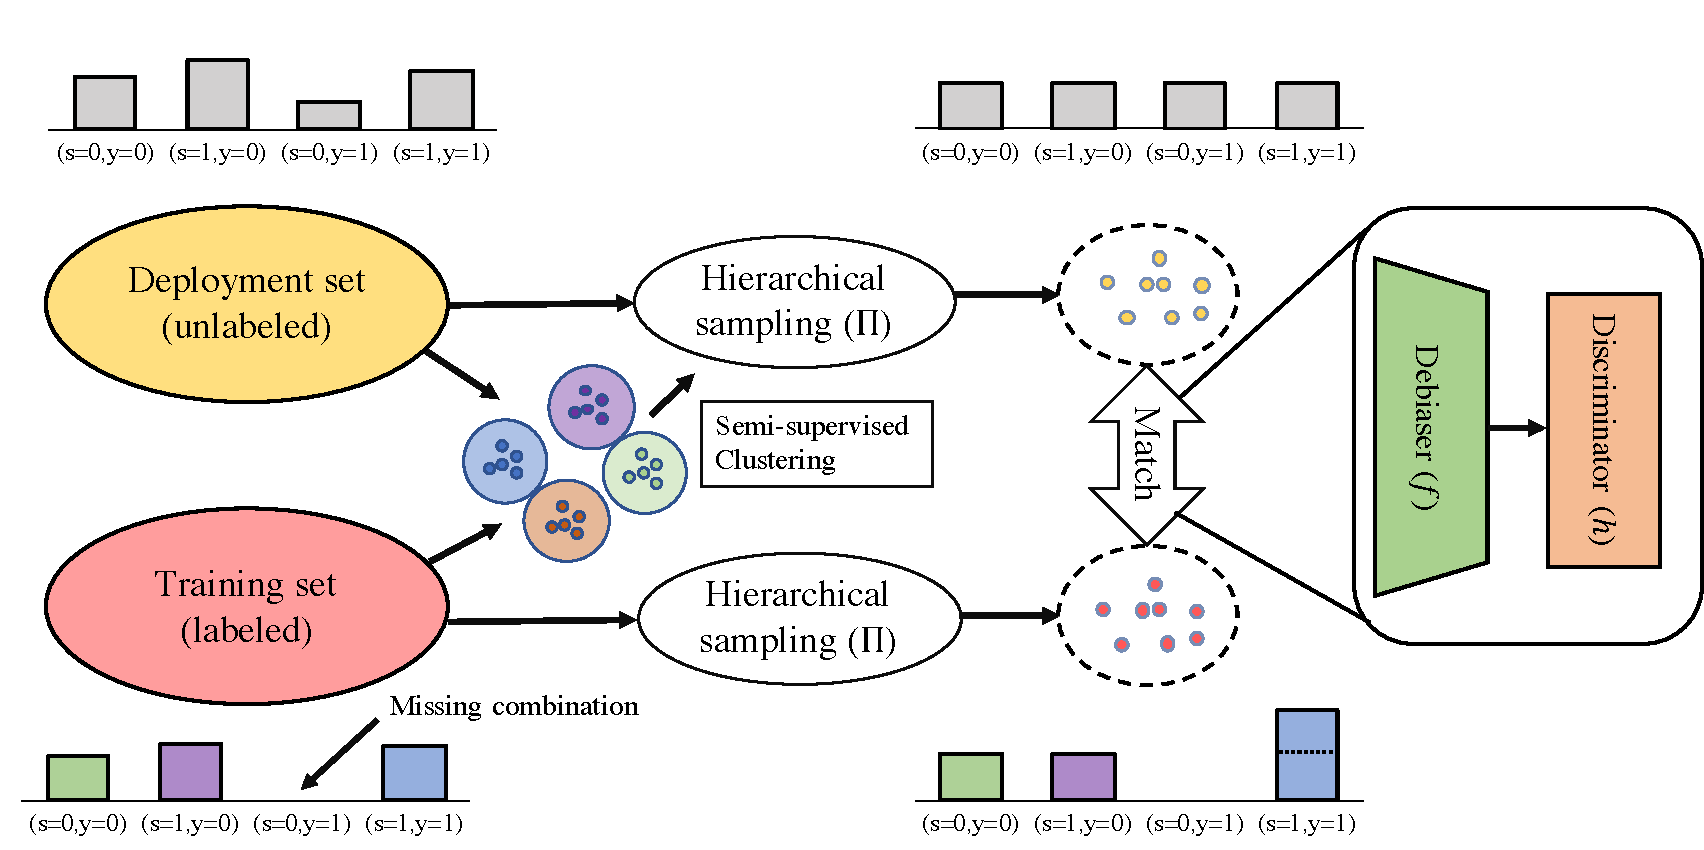
\includegraphics[width=1.0\textwidth]{supmatch/figures/illustrations/pipeline.pdf}
  \caption{%
    Visualisation of our support-matching pipeline.
    % A source is defined as certain combinations of the subgroup, s, and target class, y. Bags are
    % sampled from one of two datasets. The training set has labeled information about both $s$ and
    % $y$ but may be missing support over $S\times Y$. The deployment set on the other hand, is
    % assumed to have full support over $S \times Y$ but is unlabeled, meaning it cannot be used
    % for directly training a classifier. 
    Bags are sampled from the training and deployment sets using the hierarchical sampling
    procedure described in \S\ref{sec:sm-adversarialsm} and defined functionally in
    Eq.~\ref{eq:functional-sampling}. 
    %
    Since we cannot use ground-truth labels for hierarchical sampling of the deployment set, we use
    a semi-supervised clustering algorithm to produce balanced batches. In the event that certain
    combinations are missing, as shown here for $(s=0,y=1)$, the sampling on the training set
    substitutes the missing combinations with combinations that ensure equal representation of the
    target classes. 
    %
    The debiaser is adversarially trained to produce representations from which the source dataset
    cannot be reliably inferred by the discriminator. 
    %
    Assuming the bags are sufficiently balanced and $\gG^\mathit{tr}  \subsetneq \gG=\gS\times\gY$,
    the optimal debiaser is one that produces a representation $z$ that is invariant to $s$, which
    we prove in Appendix~\ref{implication-of-the-objective}.
    }%
  \label{fig:sm-pipeline}
\end{figure*}



We cast the problem of learning a subgroup-invariant representation as one of
\emph{support-matching} between a dataset that is \emph{labelled} but has \emph{incomplete} support
over sources, $G$, and one, conversely, that has \emph{complete} support over $G$, but is
\emph{unlabelled}. 
%
The idea is to produce a representation that is invariant to this difference in support, and thus
invariant to the subgroup. However, it is easy to learn the wrong invariance if one is not careful.
% Simply matching the distributions of the two datasets would wrongly result in the relative
% frequency of the sources being taken into account and the potential loss of task-relevant
% information.
To measure the discrepancy in support between the two distributions, we adopt an adversarial
approach, but one where the adversary is operating on small sets -- which we call \emph{bags} --
instead of individual samples. These bags need to be balanced with respect to ($s$, $y$), such that
we can interpret them as approximating $\gG$ as opposed to the joint probability distribution,
$P(S, Y)$.
%
Details on how these bags are constructed can be found in in \S\ref{ssec:realisation}
and \S\ref{sec:implementation}.
% These sets correspond to the "perfect bags" introduced in the next section,
% \S\ref{ssec:perfect-bags}:


\subsection{Objective}\label{ssec:objective}
%
We now present our overall support-matching objective. 
%
As alluded to before, the goal, in summary, is to learn an encoder, \(f\), which
preserves all information relating to $Y$, but is invariant to $S$. 
%if the training set is incomplete w.r.t.\ $s$.
Let \(P^{tr}(f(X)=z', S=s',Y=y')\) be the joint probability that a data point \(x\) drawn
from \(P^{tr}(X)\) -- the training set -- results in the encoding \(z'\) and is at the same
time labelled as subgroup \(s'\) and class \(y'\). 
%
We also define the following shorthand: $p_f(Z=z')=P^{tr}(f(X)=z')$, the distribution
resulting from sampling \(x\) from \(P^{tr}\) and then transforming \(x\) with \(f\).
%
Analogously for the deployment set: $q_f(Z=z')=P^{dep}(f(X)=z')$. 
%
For the conditioned distributions we write $p_f|_{S=s',Y=y'}$, following the convention established
in \S\ref{ssec:problem_formalism} but with the added `\(|\)' to clearly delimit the
conditioning.

The objective makes a distinction between those classes, \(y \in \gY\), for which there is overlap
with all subgroups \(s \in \gS\) in the training set and those classes for which there is not.
% An extreme version of this is when \emph{none} of the classes have overlap with a specific subgroup.
% In the \emph{missing subgroup} scenario, \emph{none} of the classes have overlap with all subgroups \(s\).
To formalise this, we define the following helper function $\Pi$ which maps \((s',y')\) to a set of
subgroup identifiers depending on whether the class \(y\) has full \(s\)-support:

\begin{align}\label{eq:Pi}
\Pi(s',y') = \begin{cases}
  \{s'\}&\text{if }\,\gS^{tr}_{ Y=y' }=\gS \\
  \gS^{tr}_{ Y=y' }&\text{otherwise.}
\end{cases}
\end{align}
%
$\Pi(s,y)$ ensures that the correct invariance is learned and is discussed in more detail further below.
Our objective is then
%
\begin{align}
  \gL_\text{match}(f)=\sum\limits_{s'\in\gS}\sum\limits_{y'\in\gY} d(p_f|_{s\in \Pi(s',y'),Y=y'},
  q_f|_{S=s',Y=y'})
\label{eq:objective}
\end{align}
%
where \(d(\cdot, \cdot)\) is a distance measure for probability distributions.
The optimal encoder $f^*$ is found by solving the following optimisation problem:
%
\begin{align}
  f^*=
  \argmin\limits_{f\in\gF} 
  \textcolor{red}{
  \gL_\text{match}(f)
  }
  - 
  \textcolor{blue}{
  \gI(f(X);X)
  }
\end{align}
%
where $\gI(\cdot; \cdot)$ again denotes the mutual information. As written, Eq.~\ref{eq:objective}
requires knowledge of \(s\) and \(y\) on the deployment set for conditioning. 
%
That is why, in practice, the distribution matching is not done separately for all combinations of
\(s'\in\gS\) and \(y'\in\gY\). 
%
Instead, we compare \emph{bags} that contain samples from all combinations in the right
proportions. For the deployment set, Eq.~\ref{eq:objective} implies that all
\(s\)-\(y\)-combinations have to be present at the same rate in the bags, but for the training set,
we need to implement \(\Pi(s',y')\) with hierarchical balancing.

As the implications of the given objective might not be immediately clear,
we provide the following proposition.
%
The proof can be found in Appendix~\ref{sec:theoretical-analysis}.
%
\begin{theorem}
%
If \(f\) is such that
%
\begin{align}
p_f|_{s\in \Pi(s',y'),Y=y'} = q_f|_{S=s',Y=y'}\quad\forall s'\in\gS, y' \in\gY
\end{align}
%
and \(P^{tr}\) and \(P^{dep}\) are data
distributions that correspond to the real data distribution \(P\),
except that some \(s\)-\(y\)-combinations are less prevalent, or, in the
case of \(P^{tr}\), missing entirely, then, for every
\(y' \in \gY\), there is either full coverage of \(s\) for \(y'\)
in the training set (\( \gS^{tr}_{ Y=y' }=\gS \)), or the
following holds:
%
\begin{align}
P(S=s'|f(X)=z', Y=y')=\frac{1}{n_s}~.
\end{align}
%
In other words: for \(Y=y'\), \(f(x)\) is not predictive of \(s\).
\end{theorem}

\subsection{Implementation}\label{ssec:realisation}
%
The implementation of above objective combines elements from unsupervised representation-learning and
adversarial learning.
% For simplicity, we follow an autoencoder paradigm for the former but any
% unsupervised/self-supervised representation learning objective could be used in place of the
% reconstruction objective.
In addition to the invariant representation $z$, our model also outputs $\tilde{s}$, in a similar
fashion to \citet{KehBarThoQua20} and \citet{creager2019flexibly}. 
%
This can be understood as a reconstruction of the subgroup information from the input $x$ and is
necessary to prevent $z$ from being forced to encode $s$ by the reconstruction loss.
%
We note that this need could potentially be obviated through use of self-supervised approaches,
but refrain from exploring this avenue in the interest of simplicity.

The model, $\Gamma$, is composed of three core modules: 
1) two \emph{encoder} functions, $f$ (which we refer to
as the ``debiaser'') and $t$, which share weights and map $x$ to $z \in \gZ$ and
$\tilde{s} \in \tilde{\gS}$, respectively;
2) a \emph{decoder} function \(r: \gZ \times \tilde{\gS} \to \gX\) that learns to
invert $f$ and $t$; and
% 3) \emph{predictor} functions $\ell_y$ and $\ell_s$ that predict $y$ and $s$
% from $z$ and $\tilde{s}$ respectively, and
3) a \emph{discriminator} function $h: \gZ \to ( 0, 1 )$ that predicts which
dataset a bag of samples embedded in $\gZ$ was sampled from. 
% The predictor $\ell_s: \tilde{\gS} \to \bigtriangleup^{|\gS|}$ (with $\bigtriangleup^{|\gS|}$
% denoting the $|\gS|$-dimensional standard simplex) is usually the identity function, and is
% primarily listed here for notational symmetry. Fig. \ref{fig:architecture} illustrates how $f$
% and $h$ interact during training -- the decoding step involving the other two components, $t$ and
% $g$, is omitted for compactness. This marks a significant departure from the typical GAN
% discriminator, which takes as input batches of data and yields a prediction for each sample
% independently of the other samples in the batch. %, where the training signal comes from the
% perfect dataset.
%
The encoder $f$ is then tasked with learning a representation $z$ such that it is indeterminable to
the adversary $h$ whether a given bag originated from the deployment set (`positive') or the
training set (`negative').
Formally, given bags
\( \gB^{tr} \), sampled according to \(\Pi\) from the training set, and balanced bags from the deployment
set, \( \gB^\mathit{dep} \), we first define, for notational convenience, the loss \wrt{} to the
encoder networks, $f$ and $t$ as
%
\begin{align}
&\gL_\text{enc}(f, t, r, h) = 
  \sum_{b^{dep} \in \gB^{dep}}
  \sum_{b^{tr} \in \gB^{tr}} 
\textcolor{blue}{
  \Bigg[\,
    \overbrace{
    \sum_{x \in b^{dep} \cup b^{tr}} 
      \lVert x - r(f(x), t(x))\rVert_p^p}^{\gL_{\text{recon}}}
    \Bigg]
    }
    \nonumber\\
   &\quad\quad\quad\quad\quad\quad
 %   +  
   \textcolor{red}{
     \underbrace{ \lambda_\text{match}  \Bigg[
       \log h \bigl( \{ \texttt{sg}[f(x)]\ | x \in b^\mathit{dep} \} \bigr) 
       - \log h \bigl( \{ f(x)\ | x \in b^\mathit{tr} \} \bigr) 
 \Bigg] }_{\gL_{\text{match}}},
}
   % \nonumber\\
   % &\quad+ \!\!\sum_{x\in b_\mathit{tr}}
   % \lambda_y L_{\text{sup}} (
   % y, \ell_y(f(x))) + \lambda_s L_{\text{sup}} (s, \ell_s(t(x)))
\label{eq:disentangling}
\end{align}
%
where \( \gL_{\text{recon}} \) denotes the reconstruction loss defined by the \(p\)-norm (\(p=1\)
and \(p=2\) yielding MAE and MSE, respectively), \( \gL_\text{match} \) denotes the adversarial loss,
\( \lambda_\text{match} \in \mathbb{R}^+_\ast \) is a pre-factor controlling the trade-off between
the loss terms, and \( \texttt{sg}[\cdot] \) denotes the ``stop-gradient`` operator that behaves as
the identity function but with zero partial derivatives.
%
The overall objective, encompassing $f$, $t$, and $h$ can then be formulated in terms of
\( \gL_\text{enc} \) as
%
\begin{align}
    \underset{f, t, r}{\textrm{min}}\; \underset{h}{\textrm{max}}\,\gL_\text{enc}(f, t, h)~.
    \label{eq:disentangling_total}
\end{align}
%
This equation is computed over batches of bags and the discriminator is trained to map a bag of
samples from the training set and the deployment set to a binary label: $1$ if the bag is adjudged to
have been sampled from the deployment set, $0$ if from the training set.
% Its goal is to effectively estimate the probability that a bag of samples has been sampled from
% one distribution or the other.
For the discriminator to be able to classify sets of samples, it needs to be permutation-invariant
along the bag dimension -- that is, its predictions should take into account dependencies between
samples in a bag while being invariant to the order in which they appear. 
% We experiment with two different types of attention mechanism for the bag-wise pooling layer of our
% discriminator, finding them both to work well.
For aggregating information over the bags, we use a self-attention-based
\citep{vaswani2017attention} pooling layer in which the query vector is averaged over the bag
dimension.
For more details see Appendix~\ref{ssec:attention-mechanism}. 
%
Furthermore, in Appendix~\ref{ssec:no-mil}, we validate that having the discriminator operate over
sets (bags) of samples rather than independent samples (with the same balancing scheme) is
essential for achieving good and robust (\wrt{} balancing quality) performance.

% Our goal is to make $z$ invariant to the subgroup $s$. However, what the adversarial loss
% actually enforces is that $z$ generates bags with the same support over $S \times Y$ irrespective
% of the dataset they were drawn from. To ensure that the disentangling aligns with our objective,
Our goal is to disentangle $x$ into two subspaces: a subspace $z$, representing the class, and a
subspaces $\tilde{s}$,
representing the subgroup.
For the problem to be well-posed, it is crucial that the bags differ only
in terms of which sources are present and not in terms of other aspects.
% with respect to the class-subgroup combinations present and not with respect to the shape of the
% underlying distribution.
We thus sample the bags according to the following set of rules which operationalize $\Pi$. Please
refer to Fig.~\ref{fig:pipeline} for a visualisation of the effect of these rules. 
%
\begin{enumerate}\label{ls:rules}
  %
  \item Bags of the deployment set are sampled so as to be approximately balanced with
    respect to $s$ and $y$ (all combinations of $s$ and $y$ should appear in equal number). 
    %
  \item For bags from the training set, all possible values of $y$ should appear with equal
    frequency. Without this constraint, there is the risk of $y$ being encoded in $\tilde{s}$
    instead of $s$. 
  \item Bags of the training set should furthermore exhibit equal representation of each subgroup
    within classes so long as rule 2 is not violated.
    For classes that do not have complete $s$-support, the missing combinations of $(s, y)$ need to
    be substituted with a sample from the same class -- i.e., if $s \notin \gS^{tr}(y)$ we instead
    sample randomly from a uniform distribution over $\gS^{tr}(y$). 
    %
\end{enumerate}

% We supplement the implicit constraints carried by the balancing of the bags with the explicit
% constraint that $z$ be predictive of $y$, which we achieve using a linear predictor $\ell_y$.
% Whenever we have $\textrm{dim}(\mathcal{S}_{tr}) > 1$, %(in our experiments this corresponds to the
% \emph{subgroup bias} setting) we can also impose the same constraint on $\tilde{s}$, but with
% respect to $s$.

\algrenewcommand\algorithmicrequire{\textbf{Input:}}
\algrenewcommand\algorithmicensure{\textbf{Output:}}
\begin{algorithm}
  \caption{Adversarial Support Matching}\label{alg:cap} 
  \begin{algorithmic}
    \Require Number of encoder updates $N^\text{enc}$, number of discriminator updates $N^\text{disc}$,
    encoders $f$ and $t$, decoder $r$, discriminator $h$, training set $\gD^{tr}$, deployment set
    $\gD^{dep}$
    \Ensure Debiaser $f$ with learned invariance to $s$
    \\

    \For{$i \gets 1$ to $N^\text{enc}$} \Comment Encoder update loop
    \State Sample batches of perfect bags $\gB^{tr} \sim \gD^{tr}$ and $\gB^{dep} \sim
    \gD^{dep}$ using $\Pi$ (Eq.~\ref{eq:Pi})
    \State Compute $\gL^\text{enc}$ using Eq.~\ref{eq:disentangling_total}
    \State Update $f$, $t$, and $r$ by descending in the direction $\nabla \gL^\text{enc}$
    \For{$j \gets 1$ to $N^\text{disc}$} \Comment Discriminator update loop
    \State Sample batches of perfect bags $\gB^{tr} \sim \gD^{tr}$ and $\gB^{dep} \sim
    \gD^{dep}$ using $\Pi$ (Eq.~\ref{eq:Pi})
    \State Compute $\gL^\text{match}$ using Eq.~\ref{eq:disentangling_total}
    \State Update $h$ by ascending in the direction $\nabla \gL^\text{match}$
    \EndFor
    \EndFor

  \end{algorithmic}
\end{algorithm}

%
\subsection{Perfect bags}\label{sec:sm-implementation}
%
A visual overview of our pipeline is given in Fig.~\ref{fig:sm-pipeline}. 
%
Borrowing from the \ac{AF} literature \citep{chouldechova17,KleMulRag16}, we refer to a bag in
which all elements of $\gG$ appear in equal proportions as a ``perfect bag'' (even if the balancing
is only approximate). 
%
Our pipeline can be broken down into two steps: 1) sample perfect bags from an unlabelled
deployment set; and 2) produce disentangled representations using the perfect bags via adversarial
support-matching as described in \S\ref{ssec:sm-realisation}.

\textbf{Constructing perfect bags via clustering.}
%
We cluster the data points from the deployment set into \( N^C=|\gG| \) clusters by applying
spherical k-means to CLIP \cite{radford2021learning} (visual) embeddings. 
%
Specifically, we use the ResNet-50 version of CLIP, finding this to work better than the ViT-based
variants. 
%
We inject labelled knowledge into the k-means algorithm by initialising the centroids of the known
sources the mean of their features in the labelled (training) data. 
%
We find this works reasonably well for the considered datasets; since, the aim of this work is to
propose a pipeline for effectively leverage unlabelled data for invariance-learning, not to set a
new state-of-the-art in clustering, we adopt this simple clustering method for a practical
proof-of-concept compared with the artificial approach of injecting noise into the ground-truth
labels. 
%
The latter procedure is useful, however, for performing a fine-grained sensitivity analysis of our
algorithm \wrt{} clustering accuracy, in that we can simulate the runs of the algorithm at
different levels of noisiness in the bag-sampling. 
%
% We present such an analysis in \S\ref{ssec:sensitivity}.
%
Given, the cluster assignments, we can then stratify the deployment set into perfect bags, to be
used by the subsequent support-matching phase.

As a result of clustering, the data points in the deployment set \( \gD^\mathit{dep} \) are
labelled with cluster assignments generated by clustering algorithm, \( C \), giving \(
\gD^\mathit{dep}_C=\{(x_i, c_i)\} \), \(c_i = C(z_i) \),
%
so that we can form perfect bags from \( \gD^\mathit{dep}_C \) by sampling all clusters at equal
rates; there is no need for application of the $\Pi$ operator since the deployment set is complete
\wrt{} $\gG$.
%
We note that we do \emph{not} have to associate the clusters with specific $s$ or $y$ labels as the
labels are not directly used for supervision.

Balancing bags based on clusters instead of the true labels introduces an error, which we can try
to bound. 
%
For this error-bounding, we assume that the probability distribution distance measure used in
Eq.~\ref{eq:objective} is the \emph{total variation distance} \(TV\). 
%
The proof can be found in Appendix~\ref{sec:sm-theoretical-analysis}.

\begin{theorem}
%
If \(q_f(Z)\) is a data distribution on \(\gZ\) that is a mixture of \(n_y\cdot n_s\) Gaussians,
which correspond to all the unique combinations of \(y\in\gY\) and \(s\in\gS\), and \(p_f(Z)\) is
any data distribution on \(\gZ\), then without knowing \(y\) and \(s\) on \(q_f\), it is possible
to estimate
%
\begin{align}
  \sum\limits_{s^\prime\in\gS}\sum\limits_{y^\prime\in\gY} TV(p_f|_{s\in
  \Pi(s^\prime,y^\prime),Y=y^\prime},
q_f|_{S=s^\prime,Y=y^\prime})
\end{align}
%
with an error that is bounded by \(\tilde{O}(\sqrt{1/N})\) with high probability, where \(N\) is
the number of samples drawn from \(q_f\) for learning.
%
\end{theorem}
%

\subsection{Limitation and intended use}
\label{sec:sm-limitations}
% First, dataset consumers should take extra care about the cost-benefit analysis of selecting particular datasets for their machine learning tasks. 
%
Although having zero labelled examples for some subgroups is not uncommon due to the effects of
systematic bias or dataset curation, we should make a value-judgement on the efficacy of the dataset
with respect to a task.
%
% {\color{red}Corrective action such as the one described in this paper or inaction should be
% recorded.}
We can then decide whether or not to take corrective action as described in this paper.
%
A limitation of the presented approach is that, for constructing the perfect bags used to train the
disentangling algorithm, we have relied on knowing the number of clusters \emph{a priori},
something that, in practice, is perhaps not the case. However, for person-related data, such
information can, for example, be gleaned from recent census data. 
%
(see also Appendix~\ref{sec:sm-overclustering} for results with misspecified numbers of clusters.)
%
% Removing this dependency through automatic determination of the number of clusters would
% generalize our method further but this line of research is beyond the scope of the current paper. 
%
One difficulty with automatic determination of the number of clusters is the need to ensure that
the small
% but salient
clusters are correctly identified. 
%
% In the case of 2-digit Colored MNIST, for example, the deployment set may contain only a small
% portion of {\color{purple}purple} fours relative to the other subgroups, meaning that the cluster
% they form can be easily overlooked by a clustering algorithm in favor of larger but less salient
% clusters (which may be sub-clusters of other digit/color combinations). 
A cluster formed by an underrepresented subgroup can be easily overlooked by a clustering algorithm
in favour of larger but less meaningful clusters.
% less salient clusters (which may be sub-clusters of other, larger, subgroups). 

